\documentclass[12pt,addpoints]{exam}
%\usepackage{enumitem}
\usepackage{amsfonts,amssymb,amsmath, amsthm}
\usepackage{graphicx}
\usepackage{systeme}
\usepackage{pgf,tikz,pgfplots}
\pgfplotsset{compat=1.15}
\usepgfplotslibrary{fillbetween}
\usepackage{mathrsfs}
\usetikzlibrary{arrows}
\usetikzlibrary{calc}
\usepackage{geometry}
\geometry{
	a4paper,
	total={170mm,257mm},
	left=15mm,
	right=15mm,
	bottom=20mm,
	top=15mm,
}
\date{March, 2023}
\pagestyle{headandfoot}
%\firstpageheadrule
\runningheader{3rd Quarter Final Examination}{}{Page \thepage\ of \numpages}
\runningheadrule
\firstpagefooter{}{}{}
\runningfooter{By Aaron G.K.}{}{Page \thepage\ of \numpages}
\begin{document}
	\title{St John Baptist De La Salle Catholic School, Addis Ababa\\
		\large Grade 10 Physics Final Examination \\
		$3^\text{rd}$ Quarter}
	\maketitle
	\begin{center}
		\fbox{\fbox{\parbox{6in}{\centering
					Notes, and use of other aids is \textbf{NOT} allowed.  Read all directions carefully and \textbf{write your answers in the answer sheet}.  To receive full credit, you must show all of your work.
	}}}	\end{center}
	{Name:\underline{\hspace{2in}}\text{     }{Roll Number:\underline{\hspace{0.5in}}\text{     }{Section:\underline{\hspace{0.3in}}{Time Allowed: \bf{2 hours}}
				\subsubsection*{Multiple Choice Questions}
				\begin{questions}
					\question What is the SI unit of the inductance? \\ \begin{oneparchoices}
						\choice $\Omega$
						\choice $\Pi$
						\choice $\Pi s$
						\choice $\Omega s$
					\end{oneparchoices}
					\question Lenz's law tells us that the induced current acts to oppose the change in flux(\& or the motion) that caused it. What is Lenz's law a result of?
					\begin{choices}
						\choice The law of conservation of energy
						\choice The quantization of charge
						\choice The dipole moment of the electron
						\choice The law conservation of mass
					\end{choices}
					\question What is the direction of the force on a current carrying wire when it is in inserted into a region of external magnetic field?
					\begin{choices}
						\choice The force is always parallel to the direction of the current flow.
						\choice The force is always parallel to the magnetic field.
						\choice The force is sometimes parallel to the magnetic field.
						\choice The force is always perpendicular to the magnetic field.
					\end{choices}
					\question Faraday and Henry both discovered electromagnetic induction independently. Which of the following is false about their observations?
					\begin{choices}
						\choice Current was induced when there was relative motion because flux changed.
						\choice Current was induced when the poles of the magnet were switched.
						\choice Current was induced when the area of the coil was changed.
						\choice Current was induced when flux was not changing.
					\end{choices}
					\question Two charges are shot into the left in a uniform magnetic field going out of the page. One of the charges is an electron and has a circular trajectory radius $r_e$. If second charge has a charge to mass ratio greater than the electron, which of the following is true?
					\begin{choices}
						\choice The second charge has a helical trajectory unlike the electron.
						\choice The second charge will have a greater radius of its trajectory than the electron.
						\choice The second charge will have a lesser radius of its trajectory than the electron.
						\choice The second charge will experience no force and will go straight through the field.
					\end{choices}
					\question In which of the following cases does self-inductance occur? 
					\begin{choices}
					\choice When the current through a circuit changes.
					\choice When a current carrying wire is moved in an external magnetic field.
					\choice When a nearby circuit's current is changing.
					\choice When a magnet is moved closer to a solenoid.
					\end{choices}
					\question What is the force of attraction per meter between two straight current carrying wires each carrying 2A of wire that are 1m apart?($\mu_0=4\pi\times10^{-7}$H/m)\\
					\begin{oneparchoices}
						\choice $8\times10^{-7}$N 
						\choice $8\times10^{-5}$N
						\choice $8\pi\times10^{-7}$N
						\choice $8\pi\times10^{-5}$N
					\end{oneparchoices}
					\question A square loop of wire is placed in a uniform magnetic field perpendicular to the magnetic lines. The strength of the magnetic field is 2 T and the side length of the loop is 1m. What is the magnetic flux in the loop?\\
					\begin{oneparchoices}
						\choice $2Wb$
						\choice $0.5Wb$
						\choice $4Wb$
						\choice $0.25Wb$
					\end{oneparchoices}
					\question  If the magnetic field strength in the question above was suddenly increased to 12 T in a span of 2 seconds, how much emf would be induced on average? \\
					\begin{oneparchoices}
						\choice 10V
						\choice 2V
						\choice 5V
						\choice 5V
					\end{oneparchoices}
					\question Which of the following factors does not affect the induced emf during electromagnetic induction? \\ \begin{oneparchoices}
						\choice Flux
						\choice Number of turns
						\choice Field strength
						\choice Type of magnet used in induction
					\end{oneparchoices}
					\question In the region just outside the north pole of a magnet, the magnetic field lines
					\begin{choices}
						\choice point away(diverge) from the south pole
						\choice go around the south pole
						\choice are less concentrated than at the north pole
						\choice point toward(converge at) the south pole
					\end{choices}
					\question What happens if a magnet is broken in to  multiple pieces? 
					\begin{choices}
						\choice The pieces will be separate north and south poles
						\choice The pieces will be small magnets
						\choice The pieces will have north poles but no south poles
						\choice The pieces will have south poles but no north poles
					\end{choices}
					\question We have seen in class that the induced emf during induction as a function of time can be expressed as $\varepsilon(t)=NBA\omega\sin(\omega t)$. How is the output emf of a generator affected if you halve the frequency of rotation of its coil?
					\begin{choices}
					\choice The output emf will be doubled.
					\choice The output emf will be halved.
					\choice The output emf will be quadrupled.
					\choice The output emf will be tripled.
					\end{choices}
					\question The plane of a square wire circuit with side 4.0 cm long is at an angle of 60$^0$ with respect to a uniform magnetic field of 1 T. The wires have a resistance of 0.1$\Omega$. If the field drops to zero in 2 s, what magnitude current is induced in the square circuit? \\ \begin{oneparchoices}
					\choice 4 $mA$
					\choice 3 $\mu$A
					\choice 4 $mA$
					\choice 3 $\mu$A
					\end{oneparchoices}
					\question A uniform magnetic field is perpendicular to the plane of a wire loop. If the loop accelerates in the direction of the field, will a current be induced in the loop?
					\begin{choices}
					\choice No, because magnetic flux through the loop remains constant.
					\choice No, because magnetic flux through the loop changes continuously.
					\choice Yes, because magnetic flux through the loop remains constant.
					\choice Yes, because magnetic flux through the loop changes continuously.
					\end{choices}
					\question Which of the following is true about the properties of a step down transformer? \\
					\begin{choices}
						\choice It increases the output power of the transformer
						\choice It increases the output voltage of the transformer
						\choice It increases the output current of the transformer
						\choice It decreases the output power of the transformer
					\end{choices}
					\question If the magnetic force on a current carrying wire is four folds smaller than the maximum possible force, what is the angle between the current carrying wire and the magnetic field? \\
					\begin{oneparchoices}
						\choice $\sin^{-1}(\dfrac{1}{2})$
						\choice $\sin^{-1}(\dfrac{1}{4})$
						\choice $\sin^{-1}(\dfrac{1}{6})$
						\choice $\sin^{-1}(\dfrac{1}{8})$
					\end{oneparchoices}
					\question The torque on a rectangular current carrying loop is $100Nm$. If we double the width of the wire, what will the new torque be? \\ \begin{oneparchoices}
						\choice $50Nm$
						\choice $100Nm$
						\choice $200Nm$
						\choice $250Nm$
					\end{oneparchoices}
					\question If an electron is moving at a speed of $1.0\times10^{6}m/s$ through a perpendicular magnetic field of $100T$, what is the magnitude of the magnetic force on the electron?($q_e=1.6\times10^{-19}C$) \\
					\begin{oneparchoices}
						\choice $1.6\times10^{-11}T$
						\choice $1.6\times10^{-9}T$
						\choice $1.6\times10^{-12}T$
						\choice $1.6\times10^{-10}T$
					\end{oneparchoices}
					\question What is the magnetic field 2m to the right of a straight current carrying wire that has a current of 5A going upwards? \\
					\begin{oneparchoices}
						\choice $5\times10^{-7}T\otimes$
						\choice $5\times10^{-7}T\odot$
						\choice $5\times10^{-6}T\otimes$
						\choice $5\times10^{-6}T\odot$
					\end{oneparchoices}
					\question What is the inductive time constant for a circuit that has an inductor that has an inductance of 20 H and a resistor of 100$\Omega$? \\
					\begin{oneparchoices}
						\choice 0.5s
						\choice 5s
						\choice 200s
						\choice 0.2s
					\end{oneparchoices}
					\question Which of the following is true about vectors and operation on vectors? 
					\begin{choices}
						\choice The sum of two vectors is always a vector.
						\choice The product of two vectors is always a vector.
						\choice The dot product of two vectors is usually a scalar but could be a vector sometimes.
						\choice Work is an example of the cross product between two vectors.
					\end{choices}
					\question The curie temperature of Cobalt is $1,121^{0}C$. Which of the following is true?
					\begin{choices}
						\choice We can heat Cobalt up to $1000^0$C and it could still behave as a magnet.
						\choice We can heat Cobalt up to $2000^0$C and it could still behave as a magnet.
						\choice The curie temperature of a ferromagnetic substance is irrelevant to its magnetic property. 
						\choice None of the above
					\end{choices}
					\question What is the inductance of a conductor if a current changing at a rate of $3A/s$ produces an emf of 27mV?\\
					\begin{oneparchoices}
						\choice 9 H
						\choice 9 mH
						\choice 0.011 H
						\choice 0.011 mH
					\end{oneparchoices}
					\question A solenoid that has a self-inductance of 40H has 100 windings. When the number of turns has been increased to 300 while keeping all the other factors constant, what will the new self-inductance be? \\
					\begin{oneparchoices}
						\choice 120 H
						\choice $\dfrac{40}{3}$ H
						\choice 360 H
						\choice $\dfrac{40}{9}$ H
					\end{oneparchoices}
					\question According to the figure below, what will the direction of the induced current be in \textbf{coil 2} when the current in the wire(\textit{which is going upwards}) is increased?
					\begin{center}
						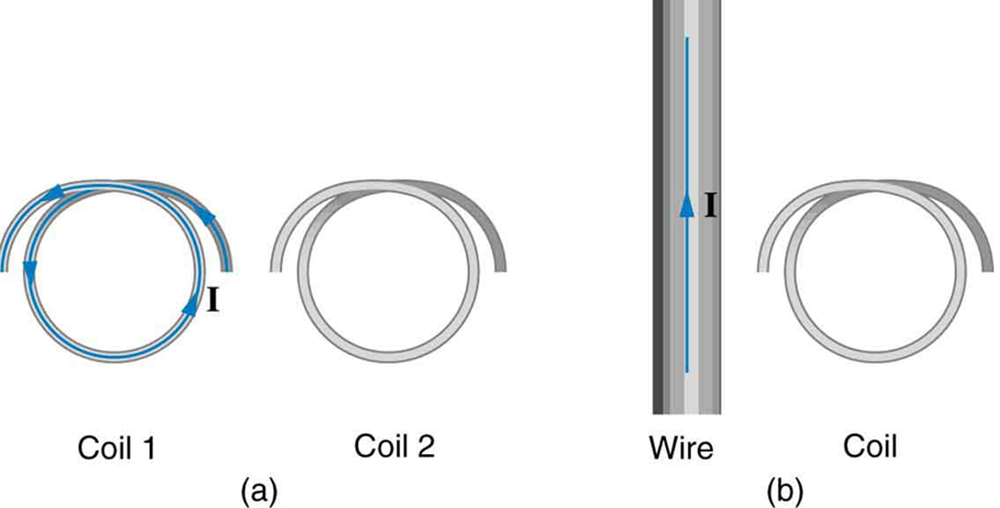
\includegraphics[scale=0.5]{coils}
					\end{center}
					\begin{oneparchoices}
						\choice Clockwise
						\choice Counterclockwise
						\choice Into the page
						\choice Upwards
					\end{oneparchoices}
					\question If $\vec{A}=2\hat{i}-3\hat{k}$ and $\vec{B}=\hat{i}-7\hat{j}-9\hat{k}$, what is the value of $\textbf{proj}^{\textbf{B}}_{\textbf{A}}\times\vec{A}$? \\
					\begin{oneparchoices}
						\choice $3\hat{i}-7\hat{j}-12\hat{k}$
						\choice 1
						\choice $5\hat{i}-7\hat{j}-12\hat{k}$
						\choice 0
					\end{oneparchoices}
					\question Which of the following is correct on the operation of the unit vectors below? \\
					\begin{oneparchoices}
						\choice $\hat{n}\cdot\dfrac{1}{2}\hat{n}=\dfrac{1}{2}$
						\choice $\hat{i}\times\hat{j}=1$
						\choice $\hat{i}\times\hat{j}=-\hat{k}$
						\choice $\hat{j}\cdot(-\hat{j})=0$
					\end{oneparchoices}
					\question Which of the following is true about charges moving in a magnetic field?
					\begin{choices}
						\choice Magnetic force is exerted when the charge is static relative to the field.
						\choice The trajectory of the particle does not depend on the entry angle of the charge and is always rectangular.
						\choice The speed of the charge has no effect on the motion and/or the trajectory of the particle.
						\choice The trajectory of the particle can be helical or circular depending on the entry angle of the charge.
					\end{choices}
					\question Which of the following is true about the difference between electric and magnetic fields?
					\begin{choices}
						\choice Magnetic fields are closed loops while electric fields don't necessarily need to be like that.
						\choice Magnetic fields can exist only from monopoles while electric fields need both parities to emerge.
						\choice Electric fields give rise to conservative fields while magnetic fields give rise to dissipative fields.
						\choice Electric fields and magnetic fields are the same.
					\end{choices}
					\subsection*{Workout Problems}
					\question Assume a 90-turn coil lies in the plane of the page in a uniform magnetic field that is directed out of the page. The coil originally has an area of  $0.050m^2$. It is stretched to have no area in 0.300 s. What is the \textbf{direction} of the current and \textbf{magnitude} of the induced emf if the uniform magnetic field has a strength of 4.50 T?\vspace{1.3in}
					\question Calculate the Hall emf induced on a patient’s heart while being scanned by an MRI unit if the conducting path on the heart wall is a wire 7.50 cm long that moves at 10.0 cm/s perpendicular to a 3.0-T magnetic field. If the hall probe has a resistance of $2\Omega$, what is current induced in the wire?\vspace{1.3in}
					\question A research solenoid at the Center for Magnetic Studies has a self-inductance of 40.0 H. 
					\begin{itemize}
						\item What \textbf{induced emf} opposes shutting it off when 100 A of current through it is switched off in 10.0 ms?\vspace{1in}
						\item How much \textbf{energy} would be stored at full current? What about when the current was decreased to 50A?\vspace{1in}
					\end{itemize}
					\question Find the \textbf{magnitude} of the magnetic field and \textbf{draw} the field lines around the following current carrying wires.
					\begin{itemize}
						\item 5m away from a vertical straight current carrying wire with 4A current going upwards.\vspace{1.5in}
						\item A 6-turn solenoid with a width of 0.50m while a current of 2A passes through it.\vspace{1in}
					\end{itemize}
					\question The wires supplying electrical power(\textit{the current in the wires are in opposite in directions}) to a commuter train in Addis carry 800 A and are separated by 80.0 cm. What is the magnitude and direction of the force between 50.0 m of these wires? Is there a risk of the wires touching?\vspace{1.5in}
					\subsection*{Extra Credit Problems}
					\question An RL circuit has an inductor of 20mH and a resistor of 20 $\Omega$ connected in series. If the circuit is connected to an emf source of 12.0 V. 
					\begin{itemize}
						\item Write the current and emf as functions of time.\vspace{0.7in}
						\item Find the induced EMF 8.00 ms after the switch is turned on.\vspace{1in}	
					\end{itemize}
				\end{questions}
				\begin{center}
					\subsection*{Answer Sheet}\vspace{0.5in}
					\begin{tabular}{lllllc}
						1.\noindent\rule{1.5cm}{0.4pt} & 6.\noindent\rule{1.5cm}{0.4pt}  & 11.\noindent\rule{1.5cm}{0.4pt} & 16.\noindent\rule{1.5cm}{0.4pt} & 21.\noindent\rule{1.5cm}{0.4pt} & 26.\noindent\rule{1.5cm}{0.4pt} \vspace{0.5cm} \\ 
						2.\noindent\rule{1.5cm}{0.4pt} & 7.\noindent\rule{1.5cm}{0.4pt}  & 12.\noindent\rule{1.5cm}{0.4pt} & 17.\noindent\rule{1.5cm}{0.4pt} & 22.\noindent\rule{1.5cm}{0.4pt} & 27.\noindent\rule{1.5cm}{0.4pt} \vspace{0.5cm} \\
						3.\noindent\rule{1.5cm}{0.4pt} & 8.\noindent\rule{1.5cm}{0.4pt} & 13.\noindent\rule{1.5cm}{0.4pt} & 18.\noindent\rule{1.5cm}{0.4pt} & 23.\noindent\rule{1.5cm}{0.4pt} & 28.\noindent\rule{1.5cm}{0.4pt} \vspace{0.5cm}\\
						4.\noindent\rule{1.5cm}{0.4pt} & 9.\noindent\rule{1.5cm}{0.4pt} & 14.\noindent\rule{1.5cm}{0.4pt} & 19.\noindent\rule{1.5cm}{0.4pt} & 24.\noindent\rule{1.5cm}{0.4pt} & 29.\noindent\rule{1.5cm}{0.4pt} \vspace{0.5cm}\\
						5.\noindent\rule{1.5cm}{0.4pt} & 10.\noindent\rule{1.5cm}{0.4pt} & 15.\noindent\rule{1.5cm}{0.4pt} & 20.\noindent\rule{1.5cm}{0.4pt} & 25.\noindent\rule{1.5cm}{0.4pt} & 30.\noindent\rule{1.5cm}{0.4pt} \vspace{0.5cm}\\              
					\end{tabular}
			   \end{center}
			\end{document}